% #############################################################################
% This is Chapter 4
% !TEX root = ../main.tex
% #############################################################################
% Change the Name of the Chapter i the following line
\fancychapter{Cooperative Motion Planning: Problem Formulation and Adopted Solutions}
\cleardoublepage
% The following line allows to ref this chapter
\label{chap:implementation}

\par In this chapter, implementation of a Direct Method based on the use of Bernstein polynomials is described. This chapter focuses on formalising the optimization problem for multiple vehicles. In chapter \ref{chap:results}, solutions for particular optimization problems are presented based on the formulations of this chapter.

\section{The Optimization Problem}
\label{sec:theoptproblem}

\par The Motion Planning problem for multiple vehicles that are the focus of this project consists of a "go-to" formation manoeuvre \cite{sabetghadam2018cooperative}. It consists of the simultaneous arrival of a formation of vehicles to desired locations whilst simultaneously avoiding collisions between each other and the environment.
\par Just as for optimization for a single vehicle, (see section \ref{sec:optimprob_intro}) motion planning for multiple vehicles will also be based on the minimisation of an appropriate cost function. Here, however, the cost will be the result of the sum of the costs of each individual vehicle and an added constraint will be necessary that will take into account inter-vehicular collisions. 

\par The optimal control formulation for this motion planning problem is defined as
\begin{equation}
    \label{eq:multi_cost}
    \begin{aligned}
    & \underset{x^{[i]}(.),u^{[i]}(.),i= 1,\dots N_v}{\text{minimize}} && \int_0^T \sum_{i=1}^{N_v}  L_i (x^{[i]}(t),u^{[i]}(t))dt + \Psi (x^{[i]}(T)) \\
    & \text{subject to}  && x^{[i]}(0) = x_0^{[i]}, \\
        & && r^{[i]}(x^{[i]}(T)) = 0, \\
        & && \dot{x}^{[i]} = f^{[i]} (x^{[i]}(t), u^{[i]}(t)), &&& t \in [0,T]\\
        & && h(x(t),u(t)) \geq 0, \\
    \end{aligned}
\end{equation}
with the same definitions as in section \ref{sec:optimprob_intro} applied to each vehicle $i=1\dots N_v$ of of $N_v$ vehicles but where $h(.)$ must also handle inter-vehicle constraints.
\par A problem that only has the integral term $\sum_{v=1}^{N_v} L_v(x^{(v)}(t),u^{(v)}(t))$ is said to be in \textit{Lagrange form}, a problem that optimises only the boundary objective $\sum_{v=1}^{N_v} \Psi_v(x(T))$ is said to be in \textit{Mayer form} and a problem with both terms is said to be in \textit{Bolza form}. An example where only the \text{Mayer form} would be necessary could be a situation where the desired destination of the vehicles does not have enough room for them all to be arranged in their desired positions. Therefore, the goal of the optimiser is to find the closest to the desired positions.

\par A direct method based on Bernstein polynomials is used here. This means that some or all of the state variables/inputs are approximated by polynomials, each with the same order $N$. By using these polynomials all of the states and inputs for each vehicle combined will produce a total of ($N_v \times (n_u+n_x)\times (N+1))$ control points.
\par Let $t_0$, $t_1$, ..., $t_N$ be a set of equidistant \textit{time nodes} such that $t_j= j\frac{t_N}{N}$, with $T>0$. By following the notation of Bernstein polynomials:
\begin{equation}
    \begin{gathered}
        x^{[i]}(t) \approx x_N(t) = \sum_{j=0}^N \overline{x}^{[i]}_{j,N} b_{j,N}(t), \quad t\in[0,T] \\
        u^{[i]}(t) \approx u_N(t) = \sum_{j=0}^N \overline{u}^{[i]}_{j,N} b_{j,N}(t), \quad t\in[0,T]
    \end{gathered}
\end{equation}
with $x_N: [0,T]\rightarrow \mathbb{R}^{n_x}$ and $u_N:[0,T]\rightarrow \mathbb{R}^{n_u}$. In this equation above, $\overline{x}_{j,N}\in \mathbb{R}^{n_x}$ and $\overline{u}_{j,N}\in \mathbb{R}^{n_u}$ are Bernstein coefficients. Let $\overline{x}_N\in \mathbb{R}^{n_x\times (N+1)}$ and $\overline{u}_N\in \mathbb{R}^{n_u}\times(N+1)$ be defined as $\overline{x}_N = [\overline{x}_{0,N},\dots, \overline{x}_{N,N}]$, and $\overline{u}_N = [\overline{u}_{0,N},\dots, \overline{u}_{N,N}]$

\par The optimization problem now becomes 
\begin{equation}
    \label{eq:multi_cost_bern}
    \begin{aligned}
    & \underset{\overline{x}_N^{[i]},\overline{u}_N^{[i]},i= 1,\dots N_v}{\text{minimize}} && \int_0^T \sum_{i=1}^{N_v}  L^{[i]} (\overline{x}_N^{[i]},\overline{u}_N^{[i]})dt + \Psi (x_{N,N}) \\
    & \text{subject to}  && \overline{x}^{[i]}_{0,N} = x_0^{[i]}, \\
        & && \overline{x}^{[i]}_{N,N} = x_f^{[i]}, \\
        & && \sum_{k=0}^{N} \boldsymbol{D}_{j,k} \overline{x}_{k,N}^{[i]} = f^{[i]} (\overline{x}_{j,N},\overline{u}_{j,N}), &&& \forall j=0,\dots,N\
        & && h(x(t),u(t)) \geq 0, \\
    \end{aligned}
\end{equation}
where $D_{j,k}$ is the $(j,k)$-th entry of the differentiation matrix $D_N = D_{N-1}E^N_{N-1}\in \mathbb{R}^{(N+1)\times(N+1)}$ that is obtained by combining the Bernstein differentiation matrix \eqref{eq:bernderivmat} with the Bernstein degree elevation matrix whose indices are given by \eqref{eq:bernsteinelevindices}.
\par What this new optimization problem means is that cost, and constraints dealt with $h(.)$ can treat the control points as actual sample of the respective polynomial functions. On the other hand, the dynamics assume that the control points are good enough approximations for the polynomial functions themselves. As a result, the equality constraint $\dot{x}=f(x,u)$ is applied to each control point instead of all infinite points of the respective polynomials.It also means that the cost can be obtained by applying the running and terminal costs to the control points.
\par Let $(x,u)$, be a feasible solution to problem \ref{eq:multi_cost}. If the the solution if is continuous, then problem \ref{eq:multi_cost_bern} admits a feasible solution too. Moreover, let $(x^*,u^*)$ be an optimal solution to \ref{eq:multi_cost_bern} and $\{(x_N^*,u_N^*)\}^\infty_{N=N_1}$ be a sequence of optimal solution to problem \ref{eq:multi_cost_bern}, it can be proven that 
\begin{equation}
    \underset{N\rightarrow\infty}{\text{lim}} (x^*_N(t),u^*_N(t)) = (x^*(t),u^*(t)),
    \label{eq:consistencytheorem}
\end{equation}
which means that the higher the order $N$ the closer to the true cost the solution is, and, as a result, the truer is the cost too. Proof for the feasibility and consistency of \eqref{eq:consistencytheorem} can be found in \cite{cichella2018bernstein}.


\section{The Log Barrier Functional}
\label{sec:logbarrierfunc}

\par A log barrier functional can be added to the cost functional such that the motion planning problem becomes unconstrained, which is preferable because solutions to unconstrained problems generally are obtained with a lower computation time. Specifically, the inequality constraints no longer become constraints and are instead moved to the cost functional by applying a log barrier functional to them.
\par An optimization problem of the form 
\begin{equation}
    \label{eq:opt_prob_without_log_bar}
    \begin{aligned}
    & \text{minimize} && \int_0^T l(x(\tau),u(\tau),\tau)d\tau + m(x(T)) \\
    & \text{subject to}  && \dot{x}(t) = f(x(t)),u(t),t),\quad x(0)=x_0 \\
        & && c_j(x(t)),u(t),t)\leq 0, \qquad t\in [0,T],j\in \{1,\dots,k \}
    \end{aligned}
\end{equation}
becomes
\begin{equation}
    \label{eq:opt_prob_with_log_bar}
    \begin{aligned}
    & \text{minimize} && \int_0^T l(x(\tau),u(\tau),\tau)+\sum_j \beta_\delta(-c_j(x(t),u(t),t))d\tau + m(x(T)) \\
    & \text{subject to}  && \dot{x}(t) = f(x(t)),u(t),t),\quad x(0)=x_0 \\
    \end{aligned}
\end{equation}
\par Given that the inequality constraint functional must be negative for the solution to be feasible, $\beta_\delta(-c_j(\cdot))$ must be nearly constant for positive values. One possible log barrier functional can be
\begin{equation}
    \beta_\delta (z) = 
    \begin{cases}
        -\log{} z & z>\delta \\
        \frac{k-1}{k}\left[\left(\frac{z-k\delta}{(k-1)\delta}\right)^k-1\right]-\log{}\delta & z\leq \delta
    \end{cases}
\end{equation}
which is continuous and whose derivative around $z=\delta$ is also continuous too. \cite{hauser2006barrier}.
\par The "hockey stick" function, with form given by
\begin{equation}
    \delta(z)= \begin{cases}
        \tanh(z), & z\leq 0 \\
        z, & z<0
    \end{cases}
\end{equation}
can be applied to the log barrier functional such that its derivative is smaller for feasible solutions when combined with $\beta$. Figure \ref{fig:logbarrierfunc} shows the log barrier function with and without the hockey functional applied.

\begin{figure}
\centering
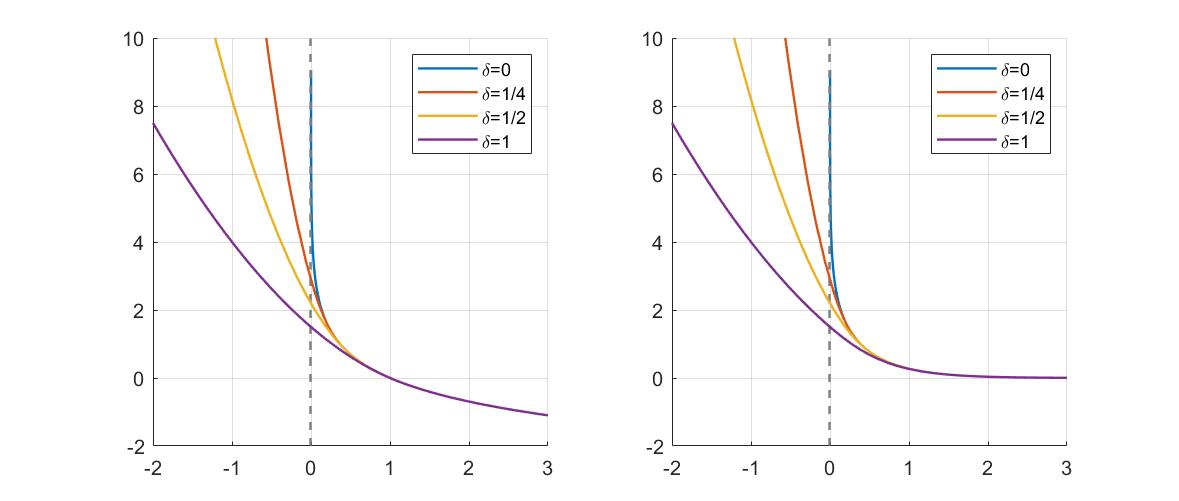
\includegraphics[width=0.8\textwidth]{Images/logbarrierfunc.jpg}
\caption{log barrier functional without (left) and with (right) the hockey stick function}
\label{fig:logbarrierfunc}
\end{figure}

\section{Inter-Vehicular Constraints}
\label{sec:mindistintveh}

\par There are 2 ways of preventing inter-vehicle collision: \textit{spatial deconfliction} and \textit{temporal deconfliction} \cite{hausler2015mission}.
Spatial deconfliction is appropriate for \ac{PF} and imposes the constraint that the spatial paths of the vehicles under consideration will never intersect and keep a desired safe distance from each other. Temporal deconfliction is appropriate for \ac{TT} and requires that two vehicles will never be ”at the same place at the same time”. However, their spatial paths are allowed to intersect. Figure \ref{fig:deconfliction} illustrates the two types of deconfliction strategies. Temporal deconfliction allows an extra degree of freedom and will intuitively lead to cheaper dynamic costs.

\begin{figure}
    \centering
    \begin{subfigure}[b]{0.45\textwidth}
        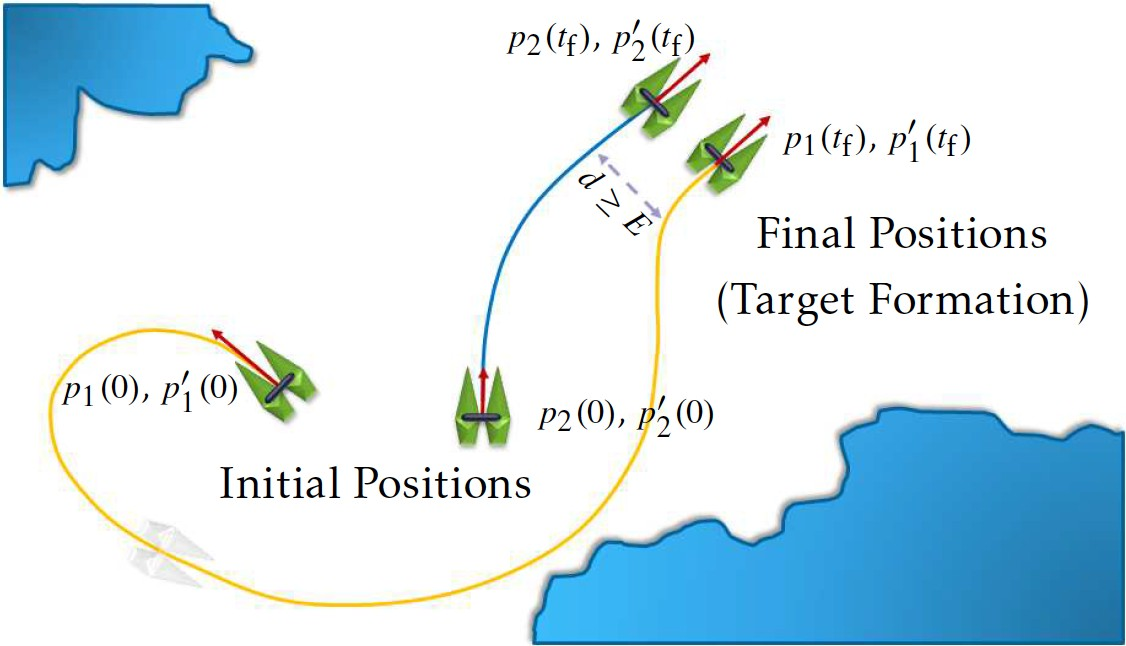
\includegraphics[width=\textwidth]{Images/spacial_deconf.jpg}
        \caption{Spacial Deconfliction}
    \end{subfigure}
    ~
    \begin{subfigure}[b]{0.45\textwidth}
        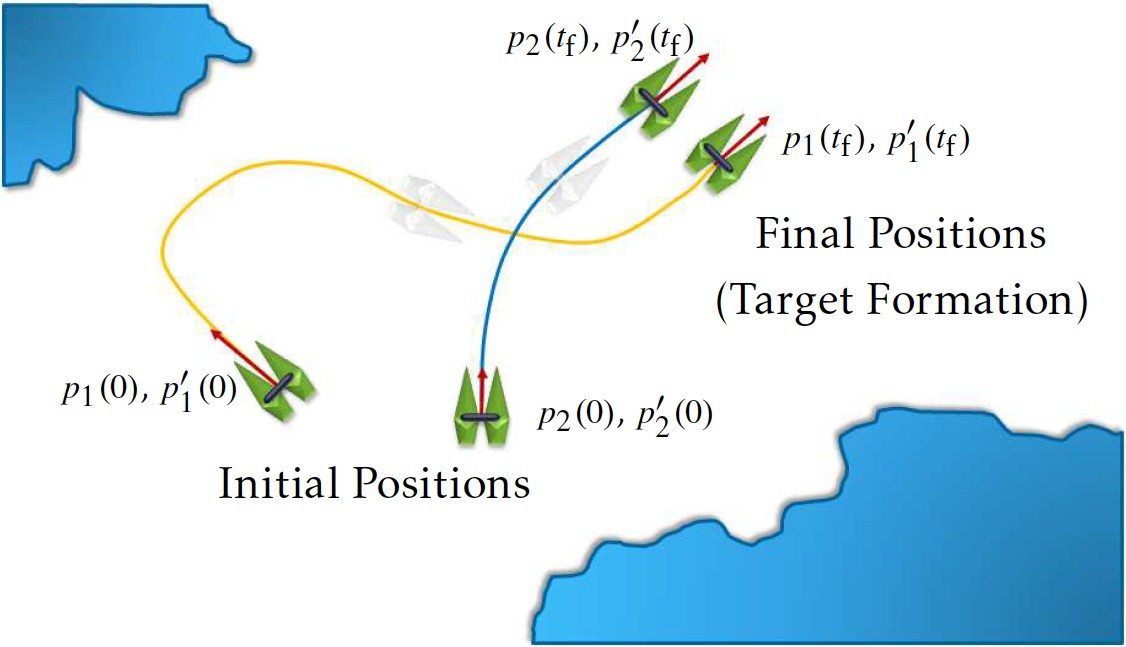
\includegraphics[width=\textwidth]{Images/temporal_deconf.jpg}
        \caption{Temporal Deconfliction}
    \end{subfigure}
    \caption{Inter Vehicle deconfliction Solutions}
    \label{fig:deconfliction}
\end{figure}

\par Two methods for temporal deconfliction are presented here, one based on sampling the curves and the other based on directly exploiting the properties of Bernstein polynomials.

\par For $N_v$ vehicles, any of ${N_v \choose 2}$ pairs could lead to a collision, which means that all pairs must be tested resulting in quadratic time complexity. This implies that finding fast algorithms to calculate the distance between each pair of trajectories becomes essential.

\subsection{Sampling Trajectories}

\par The most straightforward way to calculate the minimum distance between two trajectories is to sample each trajectory and calculate the euclidean distance between time equivalent samples; the smallest value being the minimum distance. The smallest yields the shortest distance. This method, however, is not perfect because the finer the samples, the higher the computational cost will be. However, high accuracy in the calculation of the minimum distance between trajectories in not necessary. If, besides knowing the position of the vehicle at a sample, we also know the maximum tangent speed between that sample and the next, then the distance to the other vehicle cannot deviate more than a certain determinable value between those 2 points. It will be smaller than the calculated distance if the vehicles are moving towards each other. The number of samples will determine how large this deviation can be. The optimization algorithm will stop once it finds a minimum distance that is greater than a certain value. This implies that the number of samples must be large enough such that the deviation is relatively small when compared to the desired minimum distance. 
\par For example, consider a minimum distance of \SI{1}{meter} between two vehicles which have maximum velocities \SI{1}{\meter\per\second}. At a certain moment between two samples, the vehicles could be closer to each other than they are at the samples. Consider the worst case scenario: during half of the time interval between samples the vehicles move towards each other at maximum velocity  and half the time they move away from each other as illustrated in figure \ref{fig:theworstcasescenario}. If the time sample is \SI{10}{\milli\second}, during \SI{5}{\milli\second} the vehicles can travel \SI{1}{\centi\meter} towards each other, at the relative speed of \SI{2}{\meter\per\second}, which is a \SI{1}{\percent} deviation from the established minimum distance of \SI{1}{\meter}. If the optimization problem is reformulated to guarantee \SI{1.01}{\meter} of separation, then, with samples spaced by \SI{10}{\milli\second}, a successful optimization solution guarantees a minimum distance between vehicles of \SI{1}{\meter}. which means a total of 100 samples per second of runtime.

\begin{figure}
\centering
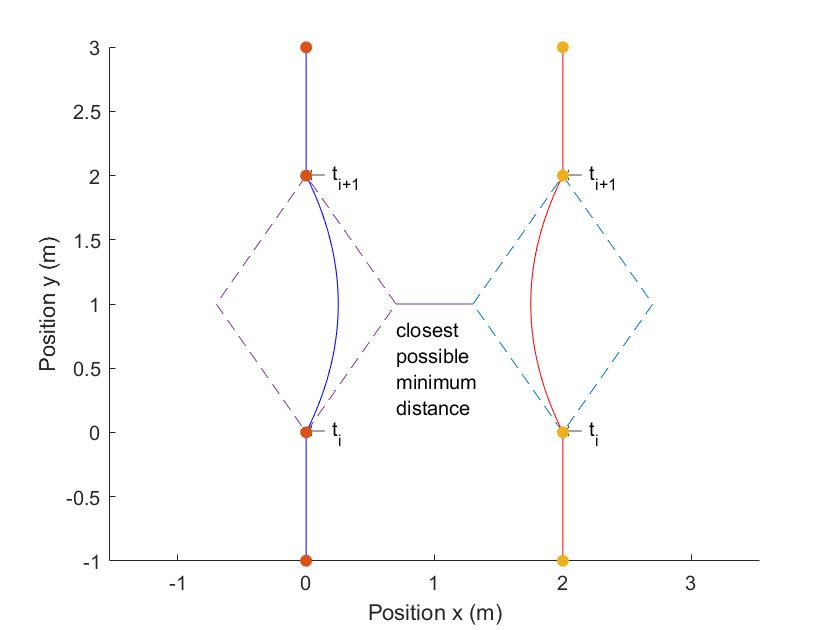
\includegraphics[width=0.8\textwidth]{Images/theworstcasescenario.jpg}
\caption{Worst case scenario for two trajectories in the time interval between samples}
\label{fig:theworstcasescenario}
\end{figure}


\subsection{Bezier Curve Distance to a Point}
\label{sec:bezcurvetopoint}

\par A second method to calculate the minimum distance between two trajectories is based on calculating the minimum distance between Bezier curves \cite{chang2011computation}. This algorithm is adapted to calculate the minimum distance between a curve and a convex shape. By subtracting the position vectors of one trajectory from the one trajectory from another, which for Bezier curves is explained in section \ref{sec:bezcurves}, finding the minimum distance between trajectories gets translated to finding the closest point of this subtraction curve to the origin which can be interpreted as a 1 point convex shape.
\par The algorithm consists of recursively breaking down the curve into two halves by obtaining a new set of control points for each half via de De Casteljau algorithm. For each half, two values are calculated: an upper and lower bounds for the minimum distance to the complex shape. The upper bound for the minimum distance will be the closest endpoint of the segment to the convex shape, the lower bound is the closest point of the convex hull of the new control points to the polygon. Both upper and lower bounds are calculated with the \acs{GJK} algorithm (see section \ref{sec:gjkalg}). The exit condition of the recursion is when the lower bound is approximately equal to the upper bound. The lower bound may be zero if the shapes intersect, which has no influence on the execution of the algorithm. If the exit condition is not met, the recursion is repeated and the returned value is the smallest of the upper bound along with the time at which the smallest value was found.

\subsection{GJK Algorithm}
\label{sec:gjkalg}

\par The \ac{GJK} algorithm \cite{gilbert1988fast} is an efficient algorithm to calculate minimum distance between arbitrary convex shapes in any dimension and is a necessary tool for calculating the minimum distance between a Bezier Curve and a point or convex shape.
\par It relies heavily on a concept called the Minkowski Sum, but, because the difference operator is used for this algorithm instead of the sum, the term Minkowski difference will be used. For two shapes $A$ and $B$, their Minkowski Difference is given by
\begin{equation}
    D = A - B = \{a-b|a\in A, b\in B\}
\end{equation}
where $D$ is a new convex shape given by the subtraction of every point in $A$ by every point in $B$.
Figure \ref{fig:intersectingshapes} shows 2 shapes on the left hand-side which intersect and the resulting Minkowski Difference on the right hand side. Figure \ref{fig:nonintersectingshapes} shows two shapes that do not intersect and their resulting Minkowski Difference. Notice how the second Minkowski Difference has an identical shape to the first, only differing on its position.
\begin{figure}
\centering
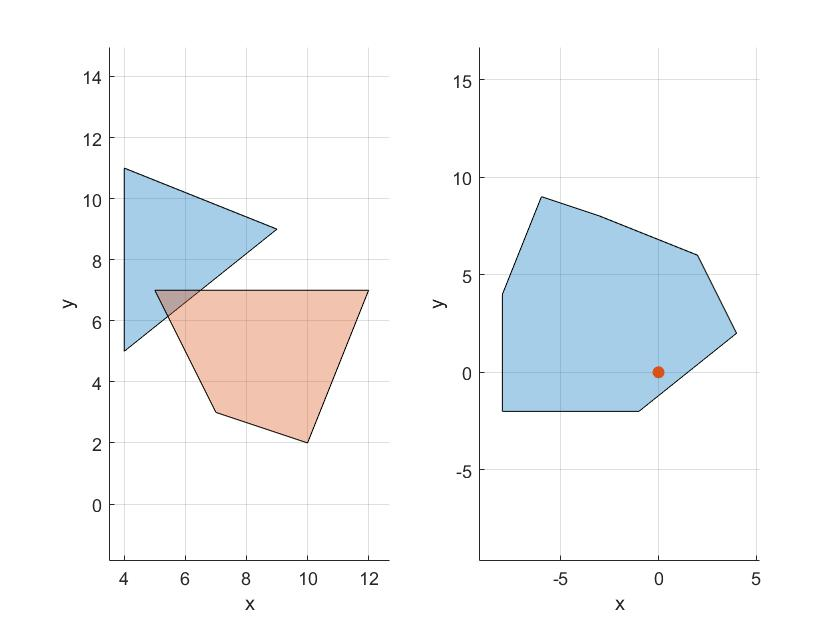
\includegraphics[width=0.8\textwidth]{Images/intersectingshapes.jpg}
\caption{Intersecting convex shapes (left) and resulting Minkowsky Difference (right)}
\label{fig:intersectingshapes}
\end{figure}
\begin{figure}
\centering
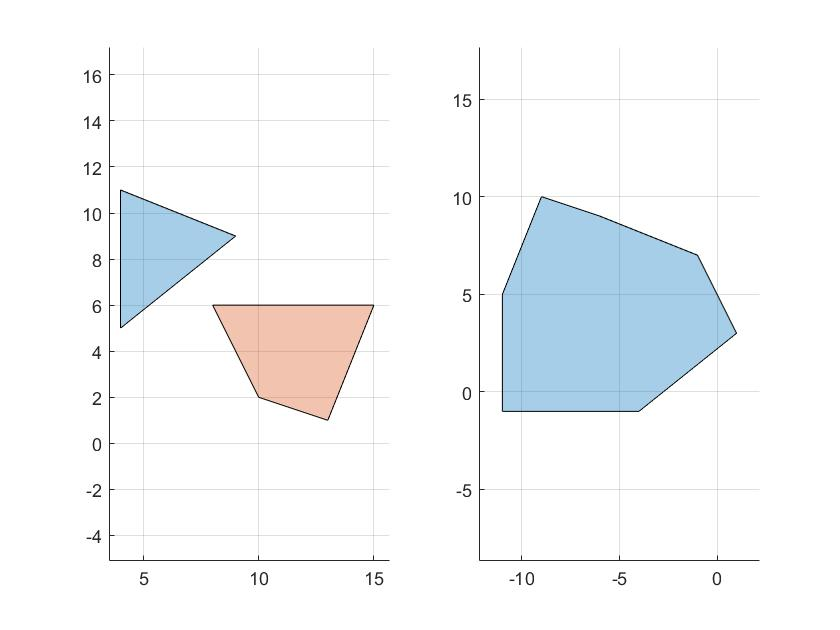
\includegraphics[width=0.8\textwidth]{Images/nonintersectingshapes.jpg}
\caption{Non-intersecting convex shapes (left) and resulting Minkowsky Difference (right)}
\label{fig:nonintersectingshapes}
\end{figure}

\par If the Minkowski Difference contains the origin, then the two shapes have common points, i.e., intersect, because the resulting subtraction is zero. It is a two part problem: 
\begin{enumerate}
    \item detect intersection, by testing if the Minkowski Difference contains the origin;
    \item if no collision is confirmed, calculate the minimum distance between the shapes.
\end{enumerate}
\par A convex shape with up to N+1 vertices in an N-dimensional space is known as a simplex. For 2-D Minkowski Differences, the simplices can be a point (1 vertex), a line segment (2 vertices) and a triangle (3 vertices). For 3-D spaces, the simplices can be the same as in 2-D spaces with the addition of a tetrahedron (4 vertices).
\par The key to \ac{GJK}'s efficiency is to find points in the Minkowski difference that are the best candidates that form a simplex that can contain the origin. 
\par A support function returns the farthest point of a convex shape in some direction. The resulting point is known as the "support" point. Finding a support point in the Minkowski Difference along direction $\overrightarrow{d}$ is the same as subtracting the support point of $A$ along $\overrightarrow{d}$ and $B$ along $\overrightarrow{d}$. 
\par Choosing the farthest point in a direction has significance because it creates a simplex which contains a maximum area therefore increasing the chance that the algorithm finishes quickly. Let $W_k$ be the set of vertices of the simplex constructed in the $k^{th}$ iteration, and $v_k$ as the point in the simplex closest to the origin. Initially, $W_0=\varnothing$, and $v_0$ is an arbitrary point of the Minkowski Difference. Since each $v_k$ is contained in the Minkowski Difference, the length of $v_k$ must be an upper bound for the distance.
\par \ac{GJK} generates a sequence of simplices in the following way. In each iteration step, a vertex $w_k = s_{A-B}(-v_k)$ is added to the simplex, with the objective of surrounding the origin. If the simplex contains the origin, then the program interrupts because the shapes intersect. If it is proven that the Minkowski Difference cannot contain the origin because the last added vertex did not move "beyond" the origin, then program interrupts and moves on to finding the minimum distance to the origin. While intersection is not proven, the new $v_{k+1}$ is perpendicular to the vector given by the last vertex with the one before that, or with the last with the third from the last, if available, depending on which has a dot product greater than 0, and the not used vertex gets removed from the simplex. Alternatively, if no intersection is proven, the new $v_{k+1}$ is the point in the convex hull of $W_k\cup \{w_k\}$ closest to the origin and $W_{k+1}$ becomes the smallest sub-simplex of $W_k\cup \{w_k\}$ that contains $v_{k+1}$.


\section{Minimum Distance to Convex Shapes}
\label{sec:mindistconvshapes}

\par Earlier, in section \ref{sec:bezcurvetopoint}, an algorithm to calculate the distance of a trajectory to a convex shape was presented. This algorithm, however, is limited to convex shapes that do not intersect with the trajectory. If the curve intersects with the convex shape, the algorithm returns zero as minimum distance. optimization algorithms, such as Sequential Quadratic Programming\cite{10.1007/978-0-387-35514-6_7}, require the derivative of the constraints to be non zero, even when the current guess for solution is not feasible because this derivate, in other words, will "inform" how far the control points must move so that the solution becomes feasible.

\par A modification to the algorithm that calculates the minimum distance to a convex shape is presented here to calculate the intersection points between the curve and the shape. Afterwards, these intersection points are used to calculate a "penetration" of the curve in the shape.
\par First thing to note is, during the recursion of the minimum distance algorithm, some endpoints of the cut segments will land inside the shape. If a segment has an endpoint inside and an endpoint outside the shape and the distance between these two points is approximately zero, then the point inside is added to a stack of intersecting points, otherwise, the recursion continues. If the control points of the recursive segments are partially in the shape while others are not, then the recursion continues, otherwise, if the control points are all outside or all inside the shape, then there is no point in continuing because the segment cannot contain any more intersection points.
% \par One thing that can be pointed out that can speed up checking if all of the control points of a segment are contained in the shape or not is by finding the convex hull of of the shape. If some control points are on the convex hull. The advantage of this way of testing if all control points are in the shape is that the complexity of the convex hull algorithm, will be $\mathcal{O}(n\log{}n)$, 
\par Once the intersection points are found, the "penetration" must be calculated. Figure \ref{fig:curveitersectingshapes} shows a curve intersecting a shape with the intersection points marked. First step is to find the convex hull of the intersection points. Once the convex hull is determined, the \ac{DEPA} explained in section \ref{sec:epaalg}  is performed with the obstacle shape along a predefined direction $\overrightarrow{d}$. The bigger the penetration depth, the "deeper" the trajectory is in the curve.

\begin{figure}
\centering
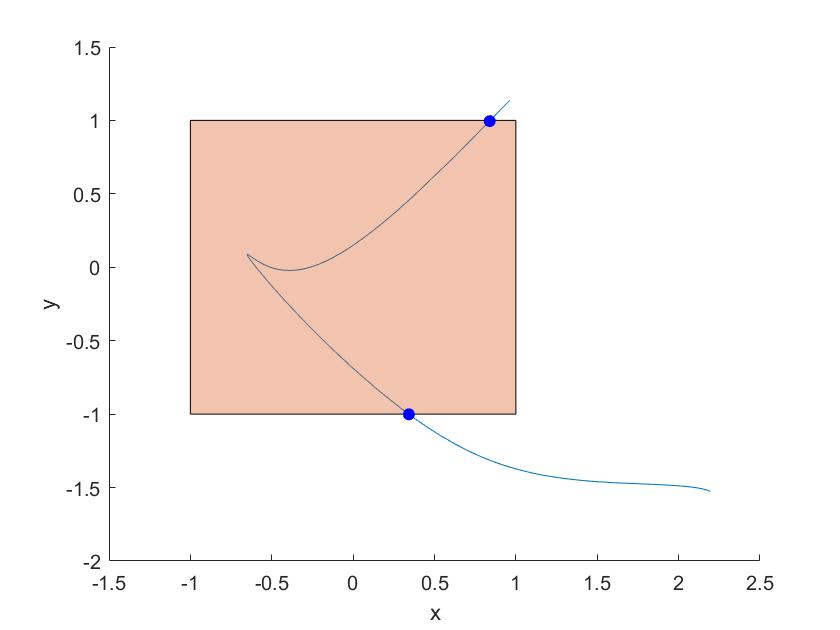
\includegraphics[width=0.8\textwidth]{Images/curveintersectingshapes.jpg}
\caption{A curve intersecting a convex shape}
\label{fig:curveitersectingshapes}
\end{figure}

\subsection{Directed EPA}
\label{sec:epaalg}

% https://graphics.stanford.edu/courses/cs468-01-fall/Papers/van-den-bergen.pdf

\par If two convex shapes intersect, the \ac{GJK} algorithm cannot provide collision information like the penetration depth and vector. One algorithm that provides this information is the \ac{EPA}.
A slight modification for the \ac{EPA} algorithm is proposed here. It will be referred as the \acl{DEPA}, whose objective is to find the penetration of one convex shape relative to another along a specific direction $\overrightarrow{d}$, while the \ac{EPA} algorithm finds the shortest vector such that the shapes no longer collide. The penetration along a direction is the length of dislocation that the second shape would have to move so that the two shapes no longer collide. 
\par The shapes intersect when the Minkowski difference contains the origin. The means that the \ac{DEPA} or the \ac{EPA} have as its objective the dislocation the Minkowski Difference such that it no longer contains the origin. Penetration along a specific direction can be found by calculating the length of the vector that starts at the origin on the Minkowski Difference, has the same direction as $\overrightarrow{d}$, and stops once it finds the edge of the Minkowski Difference. In other words, this is the norm of the intersection point between a ray starting at the origin with direction $\overrightarrow{d}$ and the edge of the Minkowski Difference. Once this length is found, shape $B$ can move by that length along the direction of $\overrightarrow{d}$ such that it is no longer in collision with shape $A$.
\par The process of looking for the penetration along a direction $\overrightarrow{d}$ starts with a simplex which contains the origin constructed with points along the edge of the Minkowski difference. The first step is to find the only edge of this polygon which will intersect with the ray that starts in the origin with direction $\overrightarrow{d}$. Once this edge is found, the other edges of the simplex are ignored and an iterative process starts. The first step of the iterative process is to calculate a vector which is normal to the current intersecting segment and points "outwards" with respect to the origin. Next, the support function is performed with this vector. The resulting point will be closer to the desired final point. There are now three points in play: the two segment ends and the new point that resulted from the support operation. The next step is to define two segments, one from the one of the segment ends to the new support point, the other from the other segment end to the support point. The next step is to find which of these two new segments intersects with the same ray with direction $\overrightarrow{d}$ and then repeat the iteration. 




\section{Soundness of Solution}
\label{sec:ivproblem}

\par Once the optimization process is complete, the trajectory is defined along with, depending on the implemented model, the control points for the inputs which can then be re-plugged into the \ac{ODE} and check what resulting trajectory is obtained, this process is known as solving an \ac{IVP}. If the approximation is good enough, the resulting trajectory should be nearly identical to the the function for the trajectory. 
\par Another strategy to check soundness is to feed the inputs to the dynamic system just as explained in the previous paragraph but, this time, a correction term is calculated as well for the inputs based on the error with the desired position, such as what is done in Trajectory Tracking.
